\documentclass[10pt]{article}
\usepackage{icmlko}

\icmlmeta{IP 파운데이션 월드모델}{156}{절반만 흔들었더니 순서가 반대였다}{노트 155가 ``판 2위가 부호를 뒤집는다''고 했다. 아니었다 --- 내 측정자가 0을 내고 있었고, 제대로 재니 판 순위와 손잡이 충실도가 $-$0.87로 어긋난다}

\begin{document}

\twocolumn[
\icmlheader

\begin{abstract}
노트 155는 축을 \emph{모든} 행에서 한 칸 올리고 예측의 평균 변화를 개입
효과로 삼았다. 순위를 내는 정식화에서 그 값은 항상 정확히 0이다 --- 단조
이동은 순위를 안 바꾸니까. F18 배깅은 그걸 알아채고 뺐는데, \textbf{F10
도메인수축도 같은 이유로 0인 것을 못 알아봤다.} 부호를 비교하니
$\mathrm{sign}(0)$ 이 $+1$ 과도 $-1$ 과도 안 같아서 일치율이 5/36 = 14\%로
나왔고, 나는 그것을 ``뒤집는 것이 규칙''이라고 적었다. \textbf{역전이 아니라
무측정이었다.} 설계를 고쳤다 --- \textbf{무작위 절반만 올리고 그 절반이
나머지에 견주어 순위가 올랐는지 본다.} 개입의 뜻과도 맞고(``이 팝업의 굿즈를
키우면 남들 사이에서 위로 가나'') 순위를 내든 눈금을 내든 똑같이 잰다.
다시 재니 \textbf{F10 은 64\%로 동전 위}이고 오히려 자료와 제일 잘 맞는다
($+$0.136). 그리고 챔피언 F18 도 이제 잴 수 있다 --- 81\%다.
\textbf{노트 155의 핵심은 살아남는다.} 다섯 정식화 전부, 모형이 함의하는
개입 효과와 그 도메인의 부분상관 사이 순위상관이 $|{\cdot}| \le 0.136$ 이다.
그런데 새로 보이는 것이 있다. \textbf{판 $\rho$ 와 ``자료 부호와 맞은 비율''
의 순위상관이 $-$0.872다.} 판 1 · 2위인 부스팅 둘(F18 · F8)이 자료 부호를
69\% · 67\%로 제일 못 맞히고, 판 4 · 5위인 선형 둘(F6 · F9)이 83\%로 제일
잘 맞힌다. \textbf{반대로 ``내 상식과 맞은 비율''은 판과 $+$0.564로 같이
간다.} 두 잣대가 갈리는 자리가 이야기다 --- 부스팅은 도메인을 건너 평균낸
강한 신호(굿즈 크면 좋다)를 배우고 그것이 상식과 맞는다. 도메인 안의 조건부
구조는 안 배우고, \textbf{손잡이에 필요한 것은 그 조건부다.}
\end{abstract}
]

\begin{figure*}[t]
\centering
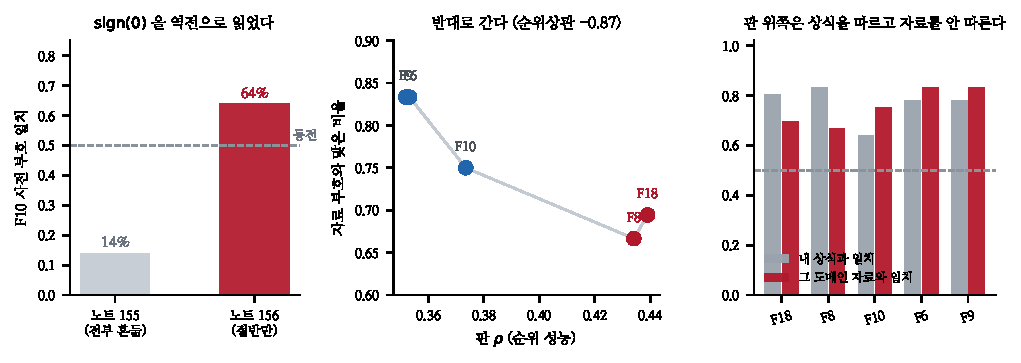
\includegraphics[width=\textwidth]{figs/half.pdf}
\caption{왼쪽 --- $\mathrm{sign}(0)$ 을 역전으로 읽었다. 가운데 --- 판
순위와 자료 부호 일치가 반대로 간다. 오른쪽 --- 판 위쪽은 상식을 따르고
자료를 안 따른다.}
\end{figure*}

\section{정정 --- 역전이 아니라 무측정이었다}

\claimx{\textbf{노트 155의 ``F10 은 부호를 뒤집는 것이 규칙(14\%)''은
틀렸다.} F10 의 \texttt{\_mix} 는 두 능형 예측을 각각 \texttt{rankdata}
로 바꾼 뒤 섞는다. 축을 모든 행에서 같이 올리면 두 순위가 다 그대로이므로
출력이 한 비트도 안 변한다 --- 평균 차가 정확히 0.0000이다.}{직접 확인했다:
세계애니 · 굿즈 규모에서 자르든 안 자르든 F10 과 F18 은 $+$0.0000, F8 만
$+$0.0641이다. \textbf{노트 155가 F18 을 뺀 그 이유가 F10 에도 그대로
있었는데 표에는 숫자가 찍히니 못 봤다.}}

\section{고친 설계 --- 절반만}

\claimx{\textbf{무작위 절반만 올리고 그 절반의 순위 이동을 본다.} 상대
순위가 실제로 바뀌므로 순위를 내는 정식화에서도 잴 수 있고, 개입의 뜻과도
맞는다.}{절반을 여덟 번 다시 뽑아 평균한다. 효과 크기가 0.033$\sim$0.039
(순위 비율 눈금)로 작지만 방향은 안정적이다.}

\begin{table}[t]
\centering\tsize
\caption{다시 잰 개입. 씨앗 셋 $\times$ 절반 여덟 번.}
\begin{tabular}{lrrrr}
\toprule
& 판 $\rho$ & 사전 & \textbf{자료} & 자료상관 \\
\midrule
F18 배깅 & \textbf{$+$.4391} & 81\% & 69\% & $-$.027 \\
F8 부스팅 & $+$.4341 & \textbf{83\%} & \textbf{67\%} & $-$.002 \\
F10 도메인수축 & $+$.3735 & 64\% & 75\% & \textbf{$+$.136} \\
F6 능형 & $+$.3532 & 78\% & \textbf{83\%} & $+$.033 \\
F9 순위우도 & $+$.3519 & 78\% & \textbf{83\%} & $+$.032 \\
\bottomrule
\end{tabular}
\end{table}

\claimx{\textbf{F10 은 64\%로 동전 위고 자료와는 제일 잘 맞는다}($+$0.136).
노트 155가 최악이라고 적은 그 정식화가 다섯 중 자료 충실도 1위다.}{그래도
$+$0.136은 작다. 순위표를 뒤집을 값은 아니고 ``제일 덜 나쁘다''는 뜻이다.}

\section{노트 155의 핵심은 살아남는다}

\claimx{\textbf{다섯 전부 손잡이가 아니다.} 모형이 함의하는 개입 효과와
그 도메인의 부분상관 사이 순위상관이 $-$0.027 $\sim$ $+$0.136이다. 제일
좋은 것도 0.14 다.}{부분상관도 인과가 아니다 --- 통제 안 된 교란이 남는다.
그러니 여기서 말하는 것은 여전히 ``자료와도 안 맞는다''까지다.}

\section{새로 보이는 것 --- 두 잣대가 갈린다}

\begin{table}[t]
\centering\tsize
\caption{판 $\rho$ 와의 순위상관. 정식화 다섯.}
\begin{tabular}{lr}
\toprule
\textbf{자료 부호와 맞은 비율} & \textbf{$-$.872} \\
자료와 순위상관 & $-$.600 \\
내 상식과 맞은 비율 & $+$.564 \\
\bottomrule
\end{tabular}
\end{table}

\claimx{\textbf{판을 잘 맞힐수록 자료 부호를 못 맞힌다}($-$0.872). 판
1 · 2위인 부스팅 둘이 69\% · 67\%, 4 · 5위인 선형 둘이 83\% · 83\%다.
\textbf{그런데 상식과는 반대로 같이 간다}($+$0.564) --- 부스팅이 상식을
제일 잘 따른다.}{정식화가 다섯뿐이라 순위상관 $-$0.872의 표준오차가 크다.
다만 부스팅 둘과 선형 둘이 깨끗하게 갈리는 것은 우연으로 보기 어렵다.}

\claimx{\textbf{읽는 법.} 부스팅은 도메인을 건너 평균낸 강한 신호를 배운다
--- ``굿즈가 크면 좋다''는 전 도메인에서 참이고 내 상식과도 맞는다. 도메인
\emph{안}의 조건부 구조(웹툰에서는 굿즈 규모가 오히려 음수)는 안 배운다.
그래서 줄은 잘 세우고 손잡이는 못 돌린다.}{노트 139가 ``풀링은 지켜 주고
희석한다''를 값으로 잡았고, 노트 148이 ``섞어도 안 오른다''를 보였다.
이 노트가 그 대가를 처음으로 손잡이 쪽에서 잰다 --- \textbf{보호받는 대신
잃는 것이 조건부 구조다.}}

\begin{table}[t]
\centering\tsize
\caption{남은 것.}
\begin{tabular}{ll}
\toprule
판정치 & 판 $\rho$ 하나로는 손잡이 쪽이 안 보인다 \\
F10 & 자료 충실도 1위 --- 도메인별 계수가 이유인가 \\
효과 크기 & 0.033$\sim$0.039 --- 한 칸이 순위를 3\%밖에 못 옮긴다 \\
\bottomrule
\end{tabular}
\end{table}

마지막 줄이 다음 자리다. 축 한 칸을 올려도 순위가 3\%밖에 안 움직인다.
사람이 매긴 축의 실제 분산이 그만큼이라면 정상이지만, 모형이 축을 거의
안 쓰고 있다는 뜻일 수도 있다. \textbf{검색 · 달력 · 위키 축이 열아홉 개고
손 축은 다섯이다} --- 그 비율부터 재야 한다.

\end{document}
